\documentclass{article}
\usepackage[utf8]{inputenc}
\usepackage{imakeidx}
\usepackage[italian]{babel}
\usepackage{graphicx}
\usepackage[T1]{fontenc}
\makeindex
\usepackage{float}
%\graphicspath{}
\title{Oscillatore di Collpits}
\author{William Perri 4427140 }
\setlength{\parskip}{1em}
\renewcommand{\baselinestretch}{1.2}
%\DeclareGraphicsExtensions{.jpeg,.png}
\date{27/06/2020}

\begin{document}

\maketitle
Insegnamento di LABORATORIO DI ELETTRONICA A.A. 2019/20

\newpage
\tableofcontents
\newpage
\section{Introduzione}
Lo scopo di questo progetto è quello di realizzare un oscillatore di Collpits, ma per iniziare dovremmo definire innanzitutto cosa è un oscillatore.
Un oscillatore (sinusoidale) è caratterizzato da:
\begin{itemize}
\item Frequenza
\item Ampiezza
\item stabilità in frequenza
\item stabilità in ampiezza
\item purezza spettrale
\item contenuto armonico
\end{itemize}
In seguito andremo ad analizzare ogni singolo punto della lista in particolar modo riferiti all'oscillatore di Collpits.
\newpage
\section{Descrizione del Progetto}
\subsection{La frequenza di oscillazione}
~\begin{figure}[H]
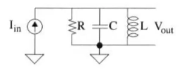
\includegraphics[scale=1]{RisonatoreParallelo.png} 
\caption{Schema circuitale di un risonatore parallelo}
\label{fig:foo}
\end{figure}
In questa figura è mostrato il risonatore parallelo, l'ammettenza del circuito vale 
$Y=G+j\omega C+\frac{1}{j\omega L}=G+j(\omega C-\frac{1}{\omega L}$ da cui $\omega_0C-\frac{1}{\omega _0L})=0 \Rightarrow \omega _0=\frac{1}{\sqrt{LC}}$ dove $\omega _0$ è la frequenza di risonanza, G è la conduttanza del resistore, gli altri due termini sono le reattanze dei due elementi reattivi.
Alla risonanza le correnti del capacitore e dell'induttore si "annullano" a vicenda,per cui dal generatore viene vista solo la resistenza. 
\subsection{La purezza spettrale}
Facendo un analisi in frequenza della forma d'onda generata da un oscillatore, dovremmo vedere una linea verticale in corrispondenza della frequenza di oscillazione e zero altrove, tuttavia questo non è possibile dal punto di vista pratico, lo spettro di un oscillatore reale mostra che c'è della potenza anche in un intorno più o meno stretto della frequenza centrale.
Questo concetto viene definito rumore di fase.

~\begin{figure}[H]
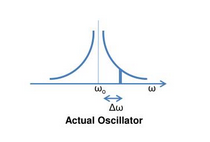
\includegraphics[scale=1]{PhaseNoise.png} 
\caption{Spettro di un oscillatore reale.}
\label{fig:foo}
\end{figure}

\subsection{Il fattore di merito}
Il concetto di fattore di merito è l'energia immagazzinata all'interno del risonatore, il momento in cui la corrente è nulla nell'induttore corrisponde a quella in cui la tensione sul condensatore è massima, l'energia del condensatore è $\frac{1}{2}CV^2$.

Quando il condensatore si scarica al minimo, la corrente dell'induttore sarà massima, per cui l'energia sarà contenuta nel campo magnetico dell'induttore determinato da $\frac{1}{2}LI^2$.
Il fattore di merito ci dice quanta di questa energia dissipiamo:

$Q=\omega\frac{EnergiaImmagazzinata}{PotenzaMediaDissipataPerPeriodo}$
\centering

Nella configurazione parallelo vista in precedenza $Q=\frac{1}{\sqrt{LC}}\frac{\frac{1}{2}CV^2}{\frac{1}{2}RI^2}=\frac{R}{\sqrt{\frac{L}{C}}}$.

Dalla prima equazione vista, ovvero quella del calcolo di $\omega_0$ partendo da L e C, e sapendo che la richiesta è far oscillare il nostro sistema a 5MHz, è stato deciso di utilizzare (tra le infinite possibilità di valori) C=100pF e L=10uH per via della facile reperibilità di questi componenti.

Con questi valori possiamo calcolarci l'impedenza caratteristica della rete:
$Z_0=\sqrt{\frac{L}{C}}=316\Omega$
\centering

Più il fattore di merito aumenta e più la curva dello spettro sarà "appuntita", il che vuol dire meno rumore di fase, un oscillatore al quarzo di buona qualità ha un fattore di merito Q=10000, un oscillatore a componenti tradizionali potrebbe arrivare a circa Q=5.

Introduciamo un nuovo concetto: la larghezza di banda dello spettro.

In questo caso si intende la banda in cui lo spettro sta dentro il range di -3dB del massimo.
Facendo un semplice calcolo è possibile vedere che il rapporto tra la larghezza di banda e la frequenza centrale è pari a 1/Q.
Ovviamente questo vuol dire che più la banda è stretta maggiore sarà il fattore di merito.
Il problema di questa realizzazione è che bisogna confrontarsi con i limiti del mondo reale, quindi la resistenza non sarà in parallelo a L e C ma la troveremo in serie a L, perché modelliamo l'induttore reale come un induttore ideale con una resistenza serie.
Ipotizziamo che $RL_S$ e $RL_P$ siano equivalenti, supponendo un Q elevato otteniamo che $R_P=R_S*Q^2$  e $L_p=L_s$.
A questo punto, ricordandoci che L=10uH, $\omega_0=2\pi * 5MHz$, la $R_s$ la andiamo a cercare su un datasheet di un induttore reale e troviamo che è circa $1\Omega$, possiamo calcolarci Q che sarà pari a 316 e per quanto detto prima $R_p=R_sQ^2=10k\Omega$.


~\begin{figure}[H]
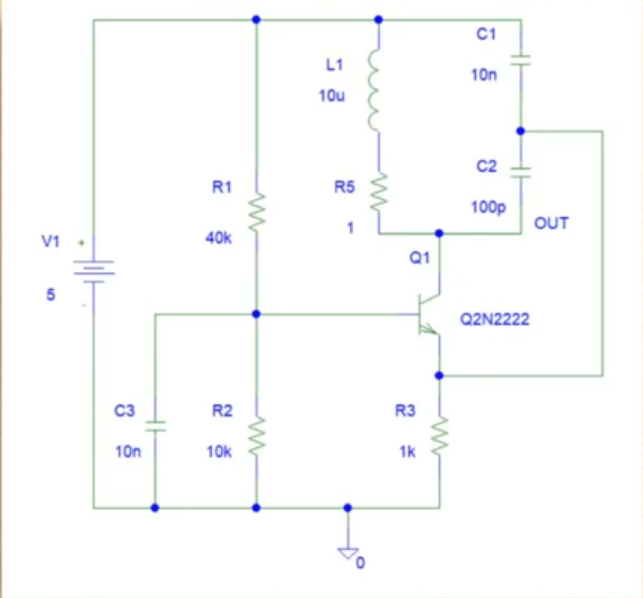
\includegraphics[scale=0.5]{Oscillatore.png}
\centering
\caption{Schema circuitale dell'oscillatore}
\label{fig:foo}
\end{figure}

Questo è il caso in cui Q=316, supponendo che il transistor sia in ZAD, il collettore ha un'impedenza molto elevata, quindi non abbiamo problemi, tuttavia la retroazione tra l'emettitore e il partitore resistivo presenta una impedenza d'ingresso dello stadio a base comune.\\
Qual è l'impedenza vista da quella porta? Andiamo ad analizzare il circuito ai piccoli segnali, ipotizzando che il segnale di ingresso $V_{IN}$ si trovi su $R_3$ con un condensatore di accoppiamento in serie.
~\begin{figure}[H]
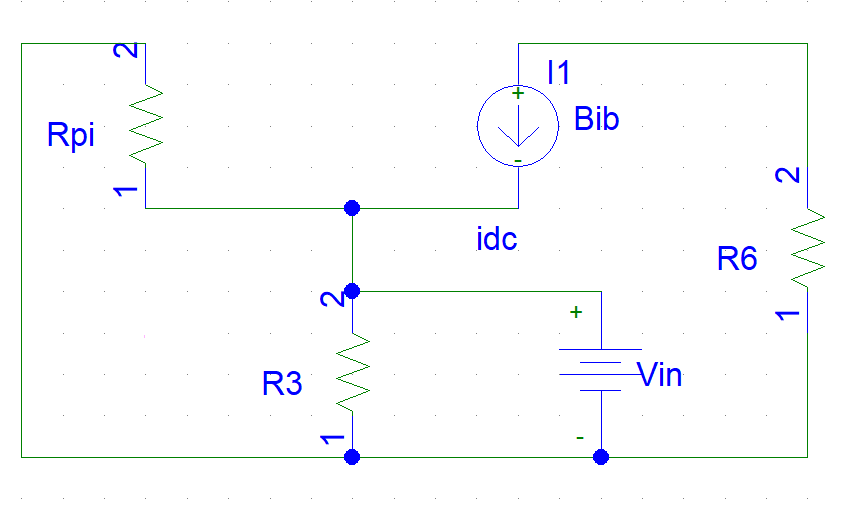
\includegraphics[scale=0.5]{PiccoliSegnali.png}
\centering
\caption{Circuito ai piccoli segnali}
\label{fig:foo}
\end{figure}
La $ib$ che pilota il generatore di corrente è ovviamente quella che scorre in $r_\pi=\frac{V_T}{I_B}=\frac{0.025}{2.6\mu }=9.6k\Omega$\\
A questo punto possiamo calcolare l'impedenza d'ingresso $Z_{IN}=\frac{V_{IN}}{i_{IN}}$\\
$V_{OUT}=- \beta i_b R_6$\\$V_{IN}=-r \pi i_b$\\
$A_V=\frac{V_{OUT}}{V_{IN}}\approx 100$\\
$i_{IN}=i_3-(\beta +1)i_b=V_{IN}(\frac{1}{R_3}+\frac{\beta +1}{r_\pi})$\\
Andando a sostituire $i_b=-\frac{V_{IN}}{r\pi}$ e $i_3=\frac{V_{IN}}{R_3}$ otteniamo che \\
$Z_{IN}=\frac{1}{\frac{1}{R_3}+\frac{\beta +1}{r_\pi}}\approx 70\Omega$
\paragraph{Prima simulazione del circuito:}
Andando a simulare il risonatore otteniamo quanto segue:
~\begin{figure}[H]
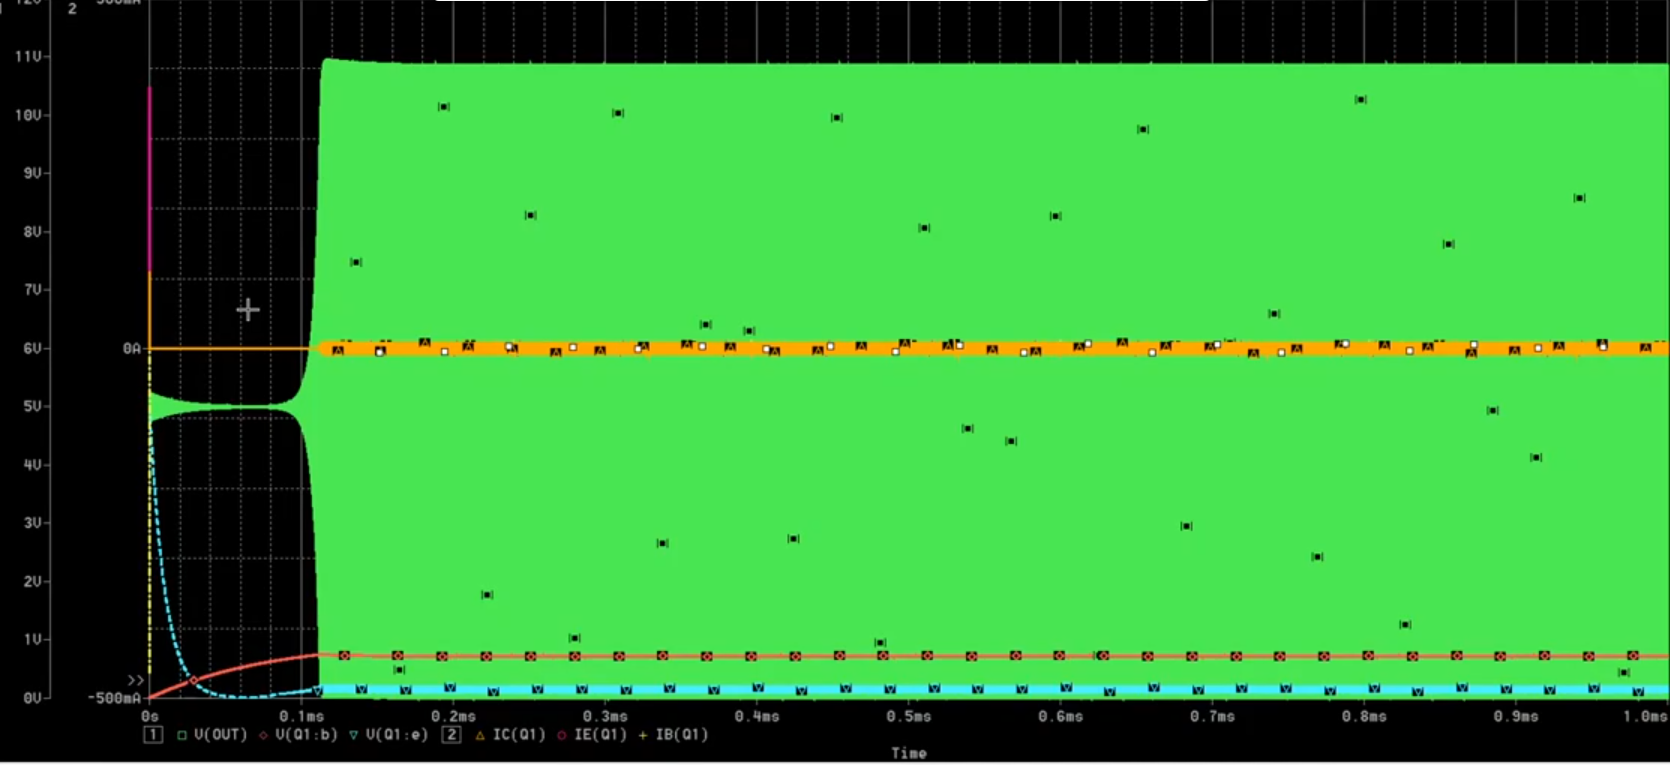
\includegraphics[scale=0.35]{RisonatoreSimulazione.png}
\centering
\caption{Simulazione nel tempo}
\label{fig:foo}
\end{figure}
Il transistor inizialmente è "spento", la linea rossa è la tensione sulla base, il condensatore C3 inizialmente è scarico, ma grazie ad R1 si carica, quando inizia a superare gli 0.8/0.9 V, fa sì che la corrente in base diventi sufficiente per polarizzare direttamente la giunzione e l'oscillazione possa iniziare.\\la tensione sull'emettitore invece inizialmente è alta perché la tensione ai capi di C1, essendo scarico, è 0V.
Quando la tensione di collettore( rappresentata in verde), tocca la tensione di base( rossa) significa che VCB=0  e quando scende al di sotto perdiamo la polarizzazione in ZAD,infatti  la tensione di collettore presenta un taglio come si può vedere nella figura 6.
~\begin{figure}[H]
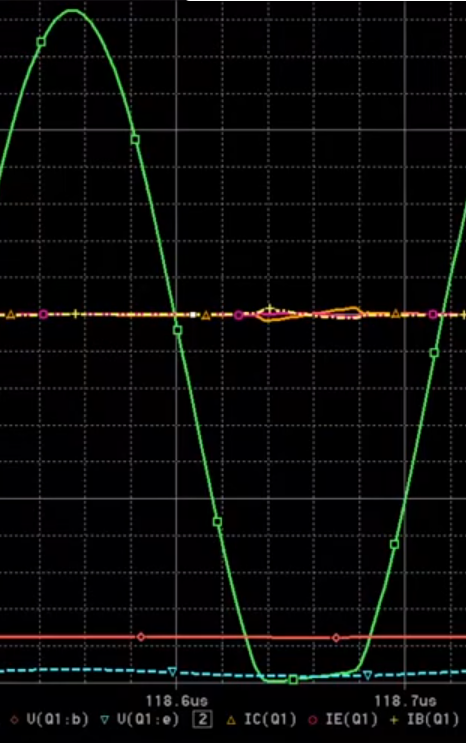
\includegraphics[scale=0.5]{SimulazioneTaglio.png}
\centering
\caption{Taglio dovuto all'uscita del transistor dalla ZAD}
\label{fig:foo}
\end{figure}
Se faccio un'analisi spettrale e calcolo la distorsione armonica totale (THD, ci indica la qualità della forma d'onda d'uscita in relazione alla potenza delle armoniche superiori in confronto all'armonica fondamentale), calcolandola riferita alle prime 4 armoniche, otteniamo un THD del 7.4\%, molto alto!\\
Questa distorsione è dovuta in gran parte al taglio che la sinusoide subisce, quindi dobbiamo aggiungere un controllo automatico dell'ampiezza per evitare che la tensione di collettore scenda al di sotto di quella di base.
Dobbiamo portare il picco massimo intorno agli 8-9V. Per questo scopo utilizziamo un raddrizzatore a singola semionda.
~\begin{figure}[H]
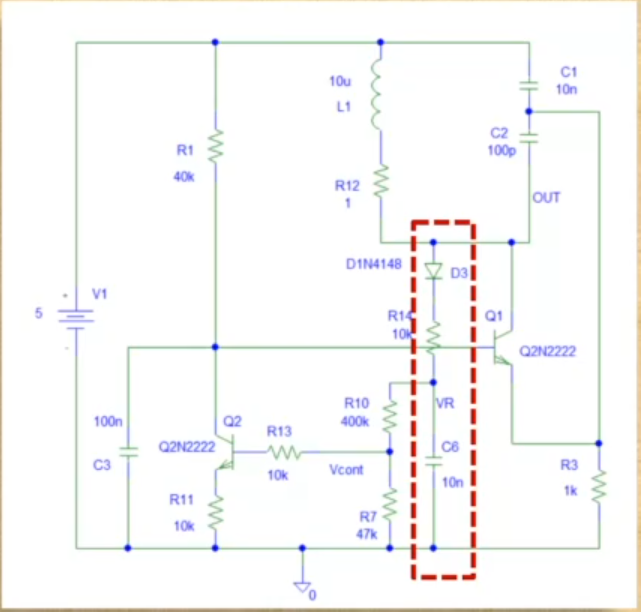
\includegraphics[scale=0.9]{RSS.png}
\centering
\caption{Circuito con il raddrizzatore a singola semionda}
\label{fig:foo}
\end{figure}
Sono stati evidenziati in figura 7 i nuovi componenti aggiunti,la R serve a caricare meno il risonatore limitando la corrente, la tensione $V_R$ sarà quella "raddrizzata" e sarà pari a $V_{MAX}-V\gamma-VR14$, la coppia R10 e R7 funziona solamente da partitore resistivo, Q2 chiude il loop di controllo, per portare il guadagno ad anello pari a 1.
Questo porta ad avere un pericolo di instabilità, all'aumentare di VR, Q2 entra in conduzione togliendo corrente alla base di Q1, facendo smettere di oscillare la tensione di collettore.
Devo introdurre un polo dominante e lo ottengo abbassando il condensatore C3 per avere un margine di fase sufficiente.
\newpage
\section{Realizzazione}

\newpage
\section{Risultati}

\newpage

\section{Conclusioni}

\newpage
\section{Riferimenti}

\begin{itemize}
\item The Design of CMOS Radio-Frequency Integrated Circuits - Thomas H. Lee
\item RF Microeletronics - B. Razavi
\end{itemize}
\end{document}
